\documentclass[a4paper, 12pt, final, garamond]{book}
\usepackage{cours-preambule}

\makeatletter
\renewcommand{\@chapapp}{Devoir surveill\'e -- num\'ero}
\makeatother

\begin{document}
\setcounter{chapter}{3}

\chapter{Commentaires sur le DS n\degree04}

\section{Commentaires généraux}
Beaucoup de sujets n'autorisent pas les calculatrices. Les aides au calcul
peuvent prendre des formes variées~: des tables de valeurs à la fin d'un sujet,
des résultats en vrac (dont des fausses pistes) au début, des aides au sein
d'une question… Il faut vous entraîner à calculer.
Concernant la mise en forme, il est généralement accepté de voir des calculs sur
une copie. Par contre,
\begin{center}
	\Large
	Pas de calcul sans unité~!!
\end{center}
Donc si vous ne voulez pas faire vos calculs sur un brouillon (faites-le),
\textit{au moins} mettez les unités.
Sinon globalement DS peu réussi. Niveau élec, il n'y a pas grand chose à
retenir~:
\begin{itemize}
	\item 1 principe~: résonance $\Lra$ amplitude max pour $\w_r \neq \{0;\infty\}$~;
	\item 2 formes de résonances~: type vitesse et type élongation~;
	\item 2 méthodes qui y sont liées~:
	      \begin{itemize}
		      \item amplitude max $\Lra$ dénominateur minimal et soit c'est évident soit
		            on dérive la fonction du dénominateur (c'est des maths…)~;
		      \item bande passante pour $X (\w) \geq X_{\max}/\sqrt{2}$ et on trouve
		            naturellement des trinômes (c'est des maths…).
	      \end{itemize}
\end{itemize}
Le reste c'est juste savoir calculer.
Niveau cinétique chimique, il y a 4 choses à connaître~:
\begin{itemize}
	\item $v = \dv{x}{t}$ avec $x$ l'avancement volumique (on retrouve le reste à
	      partir de ça)~;
	\item $v = k[\ce{A}]^{p}[\ce{B}]^{q}$~;
	\item dégénérescence/conditions stœchiométriques pour la simplifier~;
	\item la différence entre méthode intégrale/différentielle.
\end{itemize}
Même niveau «~mécanique~», les connaissances sont élémentaires~:
\begin{itemize}
	\item $\Ff\ind{Hooke} = \pm k (\ell-\ell_0)\uf$, et il suffit de déterminer
	      une longueur entre deux points (c'est du \textbf{collège})~;
	\item $m\af = \sum \Ff\ind{\ext}$.
\end{itemize}
Le reste, c'est la définition de position, vitesse et accélération, et il faut
savoir travailler avec des vecteurs (c'est des maths…).
\smallbreak
Évidemment, il faut encore savoir faire des lois des nœuds, des lois des
mailles, connaître les impédances (ou pas si vous connaissez les relations
courant-tension, il suffit de connaître la définition), ou pour la chimie il
faut encore savoir faire des tableaux d'avancement, connaître les unités la loi
des gaz parfaits, mais tout ça doit être acquis. Le détail du programme de CPGE
au début des chapitres doit vous servir à ça, les interrogations aussi.

\begin{figure}[htbp!]
	\centering
	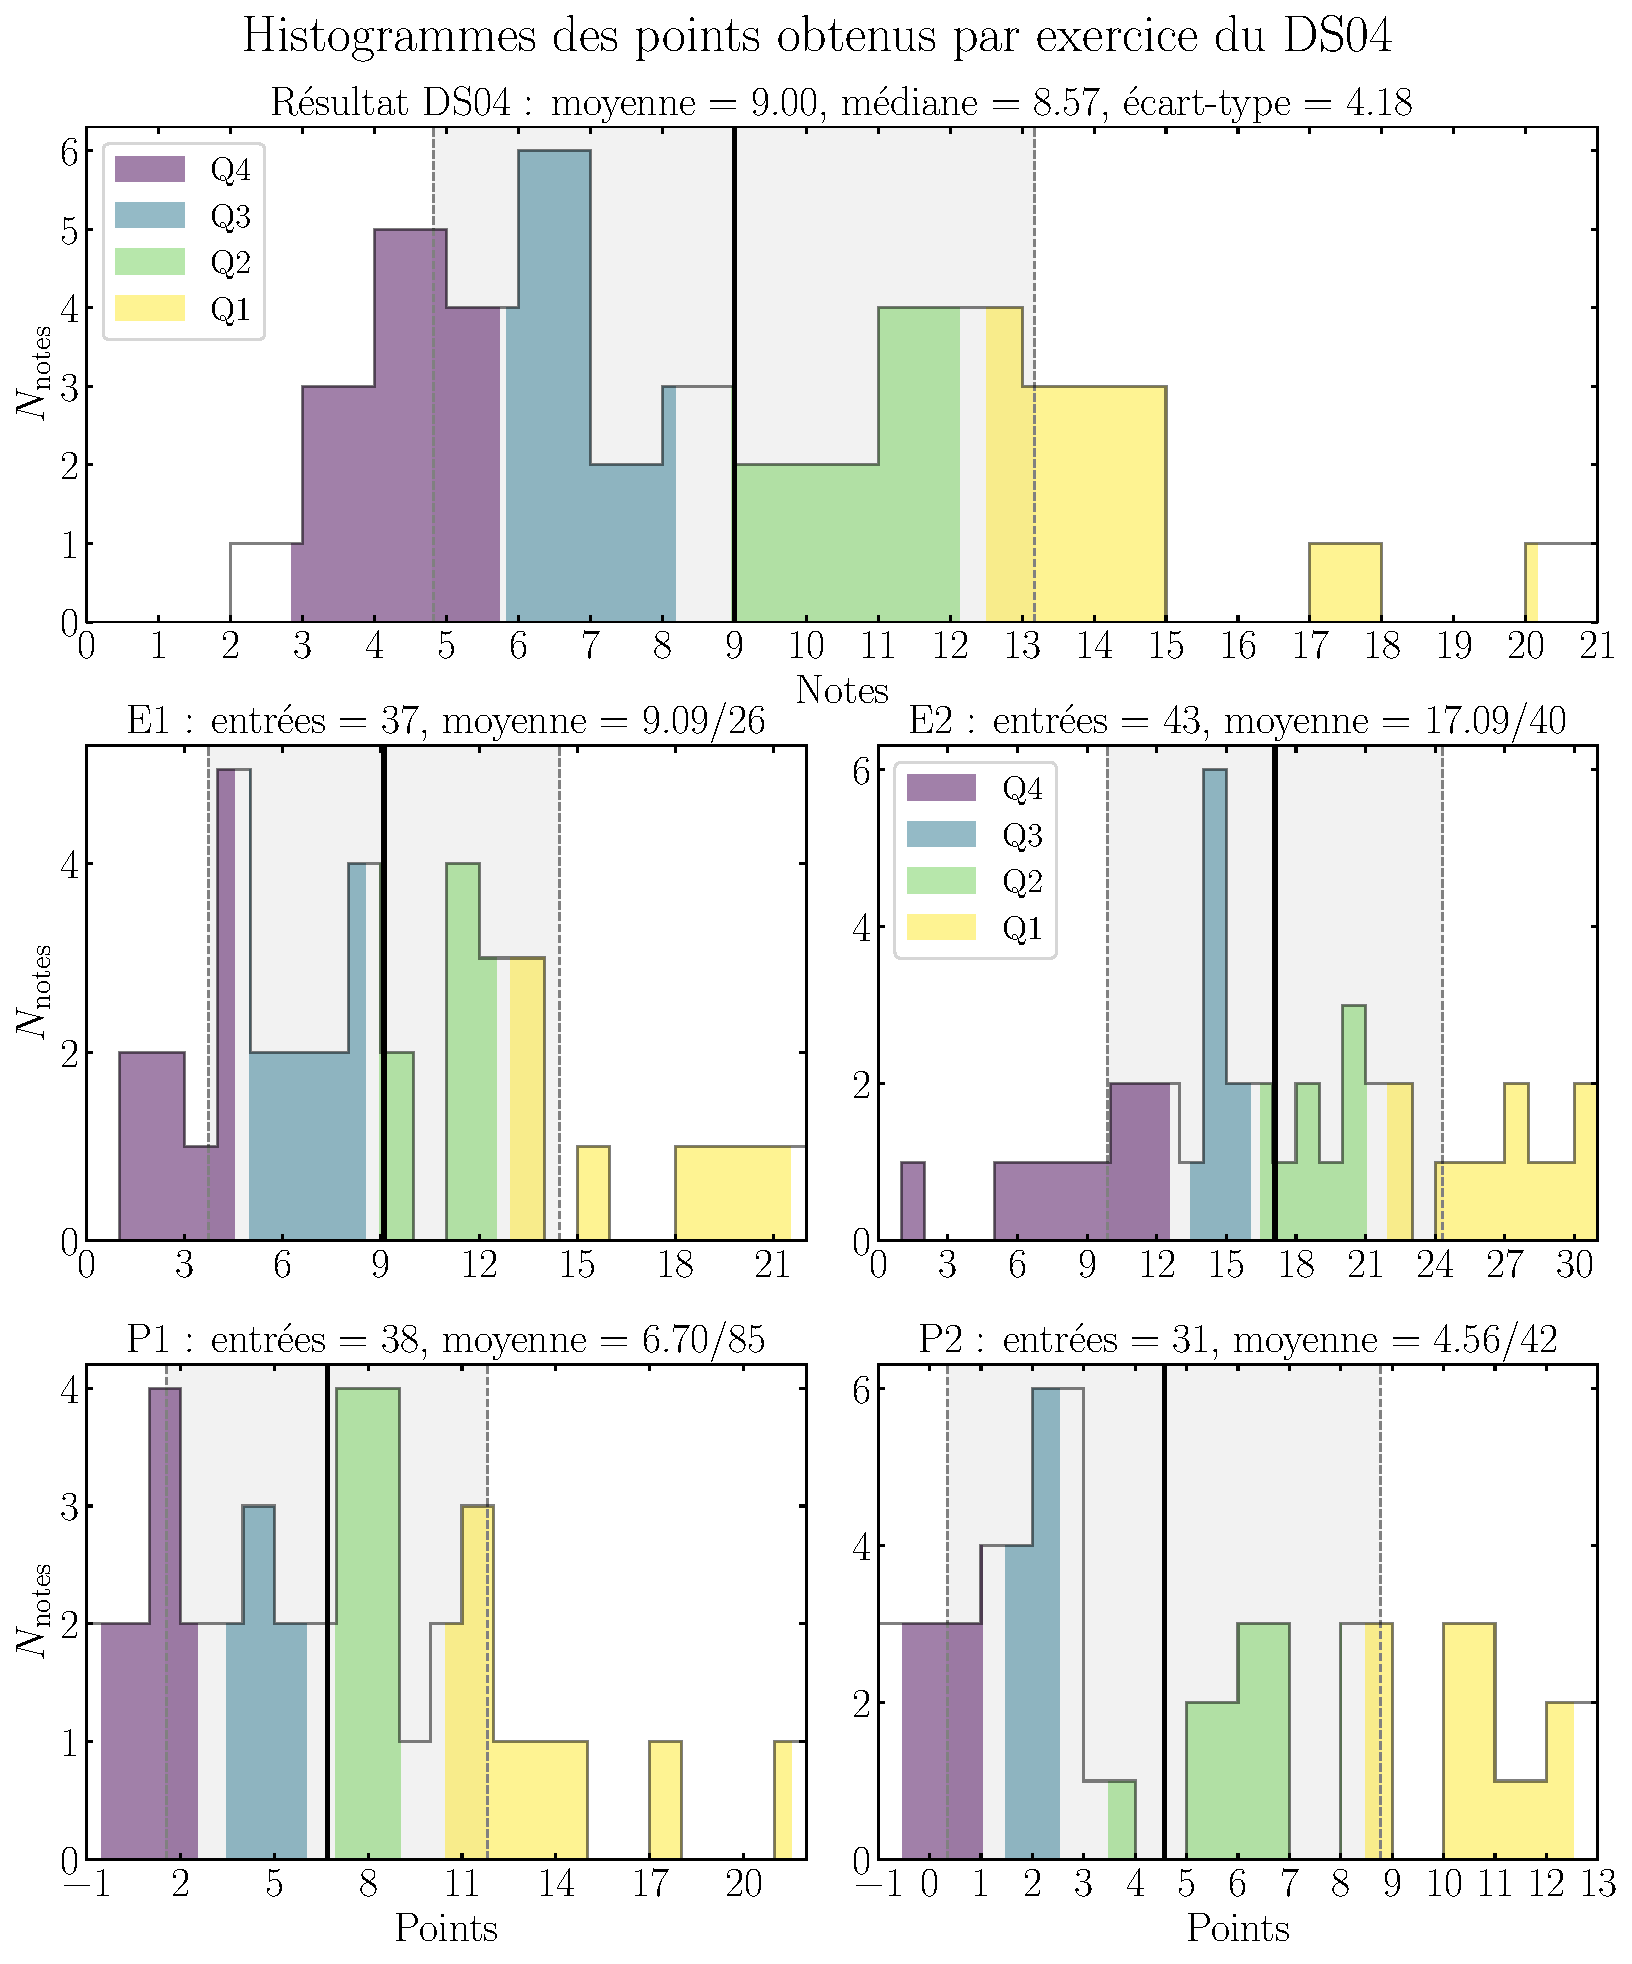
\includegraphics[width=\linewidth]{DS04_hist_all}
	\caption{Graphique des résultats}
\end{figure}

% \begin{center}
% 	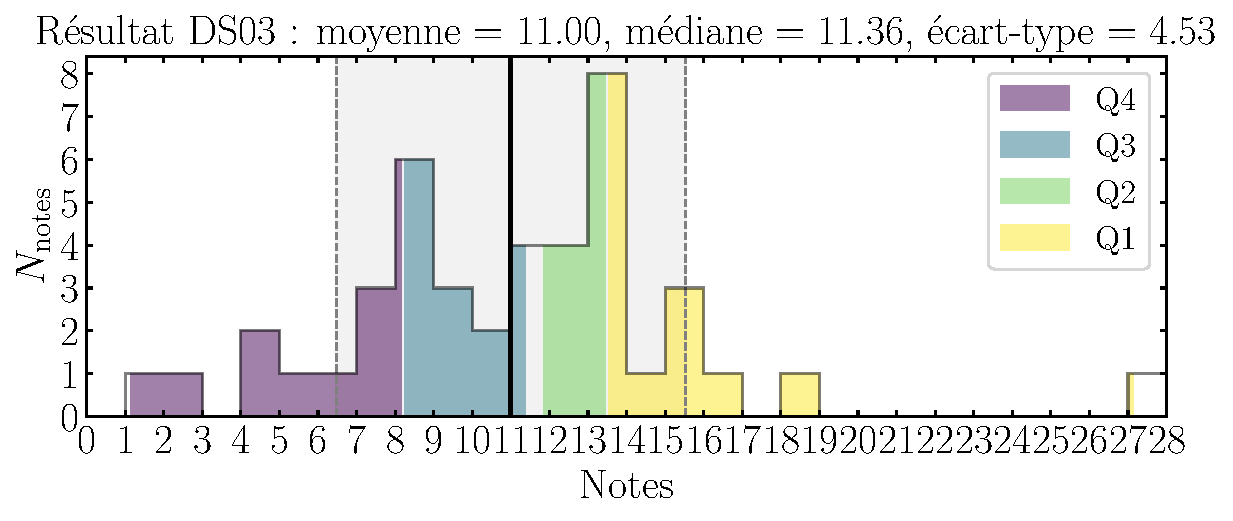
\includegraphics[width=\linewidth]{DS03_rslt.pdf}
% \end{center}

\setcounter{section}{0}
\exercice[26]{Étude cinétique de l'oxydation de la méthylhydrazine}
\begin{enumerate}
	\nitem{2}% Q1
	Trop de grosses erreurs. Il faut connaître ses définitions…
	\nitem{1}% Q2
	Bien.
	\nitem{6}% Q3
	Ok mais soyez complèt-es dans vos réponses, sans avoir à vous répéter. Pas
	besoin de refaire toute l'étude théorique avec \ce{[A]} et \ce{[B]} si vous la
	réécrivez avec \ce{[MH]} et \ce{[O2]} juste après. Par contre, justifiez
	\textit{quantitativement} l'excès de \ce{MH}. Beaucoup trop de personnes
	oublient la puissance sur la concentration du réactif en excès dans la
	constante apparente…
	\nitem{4}% Q4
	Idem, il faut connaître les méthodes et comprendre le vocabulaire. Par
	essence, la méthode différentielle n'est \textbf{pas} la méthode où on intègre
	l'équation différentielle, ça c'est la méthode intégrale. Méthode
	différentielle $\Lra$ on travaille directement sur la dérivée, i.e.\ la
	vitesse.
	\nitem{5}% Q5
	Globalement ok. Ne confondez pas $k\ind{app}$ et $k$.
	\nitem{4}% Q6
	Bof car très dépendante des autres réponses.
	\nitem{4}% Q7
	Soyez malin-es, il faut un $-$ dans la loi d'\textsc{Arrhénius} sinon
	l'exponentielle diverge.
\end{enumerate}

\exercice[40]{Comparaison de deux circuits RLC}
\begin{enumerate}
	\nitem{7}% Q1
	Assez bien.
	\nitem{5}% Q2
	Coquille dans l'énoncé, c'était bien sûr $u_b$ partout. Question trop souvent
	sautée. Encore une fois, il y a un nœud et une maille, il n'y a pas d'autre
	solution que d'utiliser les deux. En plus, si on vous propose une équation
	différentielle sans $E$ dans le second membre, il est évident que la loi des
	mailles a été dérivée. C'était en plus explicite dans l'énoncé de la question
	\fbox{5}.
	\nitem{2}% Q3
	Suivez l'énoncé~: «~à partir de l'équation~» donc pas de PdT. Globalement ok.
	\nitem{8}% Q4
	J'avais bien insisté sur le fait que «~donner~» n'est pas «~établir~» ou
	«~démontrer~», et vous avez bien suivi la consigne~: super~! L'énoncé est
	cependant mal tourné, et le barème compte la démonstration de $Q >
		\frac{1}{\sqrt{2}}$.
	\smallbreak
	Astuce de calcul~: $\frac{1}{\sqrt{2}} = \frac{\sqrt{2}}{2}$.
	\smallbreak
	Sinon, évitez de faire des fautes du style «~raisonnance~» ou
	«~résonnance~» ou autres, alors que le mot est écrit sur l'énoncé…
	\smallbreak
	C'est grave de confondre résonance, amplitude, pulsation, temps. Les
	incompréhensions sont profondes.
	\nitem{2}% Q5
	Ok.
	\nitem{3}% Q6
	Quelques grosses cata, problèmes d'homogénéité, et surtout des atrocités du
	style de
	\[
		\Zu\ind{eq} = \frac{1}{\frac{1}{\jcw}+\jlw} = \jcw + \frac{1}{\jlw}
	\]
	Ce qui revient à écrire
	\[
		\frac{1}{2+3} = \frac{1}{2} + \frac{1}{3}
	\]
	donc en plus d'être inhomogène c'est une erreur de calcul de collège…
	\nitem{2}% Q7
	Grosses confusions mais ok.
	\nitem{5}% Q8
	Bien.
	\nitem{6}% Q9
	Très peu répondue.
\end{enumerate}

\setcounter{section}{0}
\prblm[85]{Suspension d'un véhicule}
\begin{enumerate}[leftmargin=20pt]
	\nitem{3}% Q1
	Plein de tentatives de réponse avec l'aide au calcul, mais si la réflexion
	vitesse/période n'y est pas ça n'est pas valide.
	\nitem{7}% Q2
	\textbf{Oula}. J'ai rajouté la question «~sur quoi repose le système~» mais
	même avec ça il y a des réactions du support partout et des forces
	excitatrices magiques. Encore trop d'oublis de la longueur à vide $\ell_0$…
	J'ai rajouté la réponse pour la force de frottement (sinon il fallait la
	démontrer) pour vous guider sur le fait que la longueur était $z_G - z_S$.
	Encore une fois, des variables $x$ introduites sans aucun sens, et des vecteurs
	colonnes tout à fait magiques eux aussi. Pourquoi changez-vous la masse en $m$
	quand elle est écrite $M$~?
	\nitem{3}% Q3
	Beaucoup de fumisterie sur cette question.
	\nitem{2}% Q4
	Et là le bât blesse.
	\item[5-9)]\gpts{22}\/% Q5
	      RAS (NR).
\end{enumerate}
\begin{enumerate}[start=10, leftmargin=20pt]
	% \nitem{5}% Q6
	% \nitem{2}% Q7
	% \nitem{4}% Q8
	% \nitem{3}% Q9
	\nitem{5}% Q10
	Bof. Trop de $L$ transformés en $C$ par rapidité.
	\nitem{7}% Q11
	Quelques bonnes réponses pour celleux qui s'y sont essayé.
	\item[12-18)]\gpts{36}\/% Q12
	      NR.
	      % \nitem{4}% Q13
	      % \nitem{2}% Q14
	      % \nitem{8}% Q15
	      % \nitem{8}% Q16
	      % \nitem{5}% Q17
	      % \nitem{5}% Q18
\end{enumerate}

\prblm[42]{Cinétique de \ce{CaCO3}~: dissolution du calcaire et coraux}
\begin{enumerate}
	\nitem{4}% Q1
	Il faut un peu de détail. Traduisez «~totale~».
	\nitem{1}% Q2
	Sérieusement. La loi des gaz parfaits. Trop de fautes.
	\nitem{6}% Q3
	Attention à bien lire l'énoncé~: ici l'énoncé appelait $x$ l'avancement
	\textbf{pas volumique}~! Sinon cf.\ son unité dans le tableau. Faire un
	tableau d'avancement est indispensable (que ce soit ici ou dans la suite).
	\nitem{4}% Q4
	Ok.
	\nitem{1}% Q5
	RAS.
	\nitem{1}% Q6
	RAS.
	\nitem{5}% Q7
	Bof.
	\nitem{4}% Q8
	Idem.
	\nitem{6}% Q9
	Pire.
	\nitem{5}% Q10
	C'était subtile mais il faut voir la non-aléatoirité des données pour la
	courbe 2 (et évidemment pour la 1).
	\nitem{5}% Q11
	Haha.
\end{enumerate}

\end{document}
